\chapter{Content Chapter}
\label{sec:Content Chapter}


\section{Research Methodology}
\label{sec:Research Methodology}

Research methodology refers to the structured approach a researcher utilizes to explain and solve a research problem. For this project, a design research methodology will be utilized to solve the problem. 

\vspace{0.5cm}
\noindent
The problem for this skripsie, is to create a low-budget laparoscope. This laparoscope will be used in tests, for medical robots, and not on alive patients, rather, it will be used on phantoms. Therefore, the laparoscope should not be made out of medical grade equipment, but should functional similar to a medical laparoscope. 

\vspace{0.5cm}
\noindent
Since this project requires a design research methodology to be completed, there is a structure that can be followed. The initial phase that needs to be completed is a design requirement phase. In this section it required to determine:

\begin{itemize}
    \item Stakeholders;
    \item Design independent parameters;
    \item Boundary between wider system of interest and narrower system of interest;
    \item Functional Requirement;
    \item Non-functional Requirements;
    \item Technical performance measures;
\end{itemize}

\noindent of the system. It is essential to remain neutral in this section.

\vspace{0.5cm}
\noindent
The second phase that needs to be completed is the concept development phase. In this section, concepts are developed and described to meet all the requirement in the design requiremnet phase. These concepts are evalauted before the best concept or combination of concepts is selected. The selected concept(s) is refined further, before a final evaluation is performed.

\vspace{0.5cm}
\noindent
The last 2 sections of this methodology is the detail design and analysis phase and the evaluation phase. The detail design and analysis phase requires the researcher to usitlize the refined concept from the preceding section and create a detail design of the concept. This process does require an iterative process to create the final design. A drawing pack is required at the end of this phase that will be evaulated. The evaluation phase consist of evaluating the developed product. This includes building the product, before it can be tested. Based on the test results of the product, an evaluation can be conducted.


\section{Workplan}

This section of the proposal covers the planned workload that will be conducted for this project. As establised in the prior section, \textit{\hyperref[sec:Research Methodology]{Research Methodology}}, this project will follow a design research methodology. Therefore, it can be assumed that the project will require these following activities:

\subsection{Literature Review}

Study the literature of laparoscopic surgery to gain an understanding of the conditions that a laparoscope will experience. Consequently, there will be required to study literature that will inform what attributes the developed laparoscope should satisfy, to be used for testing purposes on future projects.

\subsection{Component Review}

Study and identify the components that can be utilized for this project. The developed laparoscope is dependent on the specifications of the acquired hardware. Therefore, a review is necessary to acquire the highest-performing components at reasonable cost.

\subsection{Compile Design Requirements for Laparoscope}

Determine the requirements for the developed laparoscope. Specify a set of evaluation criterias to determine the best concept during the concept generation phase.

\subsection{Generate Concept Design for Laparoscope}

Describe, formulate and design multiple concepts to meet the design requirements. The derived concepts is to be compared and evaluated. Afterwards the highest performing concept, or combination of concept, will be selected for a refinement and final evaluation.

\subsection{Finalise Detail Design for Laparoscope}

Design and finalise the selected concept design of the laparoscope. This includes producing relevant calculations and analysis of the developed laparoscope and the full drawing pack of the laparoscope.

\subsection{Compile Design Requirements for Test Station}

Determine the requirements for test station of the laparoscope. These requirements include a list of functionality test that should be performable on the test station. 

\subsection{Generate Concept Design for Test Station}

Describe, formulate, articulate and design the various tests required for the test station. These tests are to be evalauted and selected based on threshold value they should meet. All the selected tests will then be implemeted in a final test station concept, which upon completion would be evaluated. 

\subsection{Finalise Detail Design for Test Station}

Articulate and design the final test station for the laparoscope. This includes producing a safety report of the test station, instruction documents of how the various test should be performed and a full drawing pack of the test station.

\subsection{Construct and Implement Laparoscope}

Construction of the developed laparoscope should be conducted. This includes all software implementation and building of the developed product.

\subsection{Construct Test Station}

Construc the test station for the laparoscope. This entials all building requirements of the test station.

\subsection{Perform Functionality Test}

Perform the functionality tests of the built laparoscope. This includes following all test instructions and post processing of the results.

\subsection{Evaluate Laparoscope}

Evalaute the performance of the developed laparoscope. 

\subsection{Documentation}

Document the entirety of the project. All relevant literture review, design specifications, concept designs, test procedures, results and evaluation should be thoroughly documented. At predetermined dates, it is required to produced relevant docements, including the progress report, preliminary report and final report. 

\section{Resource Requirements} 

There are various equipment, components and lab access required to complete this project. As mentioned in the literature review's section, \textit{\hyperref[sec:Available Hardware Components]{Available Hardware Components}}, there are 2 main hardware components required for this project. However, there are various hardware components required for this project:

\begin{itemize}
    \item Single board computers.
    \item Camera Module.
    \item Display screen or monitor.
    \item Power supply.
    \item Electronical components.(Resistors, Light-emmiting diode(LED), wires, buttons)
\end{itemize}

There will also be required to manufacture a selection of parts for the laparoscope and test station. These parts will mainly consist of 3D printed parts and 1 thin walled rod with a diameter of less than 10 mm.

There will be access required to the mechanical and mechatronic labatories, to build, program and test the final product.

\section{Expected Results}

The expected results of this project, is to have a low-cost, functional laparoscope at the end of the project. To classify as a low-cost, funtional laparoscope, the laparoscope should meet these requirements:

\begin{itemize}
    \item The laparoscopes rod and camera assembly should fit within a 10 mm diameter hole. 
    \item The caputered real-time digital images should allow the operator to accurately coordinate the equipment.
    \item During testing, the laparoscope should meet a minimum required pass rate of 80\%.
\end{itemize}

\newpage
\section{Project Schedule}  

\begin{figure}[H]
    \centering
    \includegraphics[page=10, width=\textwidth, keepaspectratio]{gantt_chart.pdf}
    \caption{Skripsie Gantt Chart}
    \label{fig:gantt}
\end{figure}

\section{Risk Assessment}

This section of the proposal will cover all relevant risks of this project. Risk is an important feature of any project that needs to be maintained and mitigated to prevent the project from failling. 

\vspace{0.5cm}
\noindent
The first class of risk that will be discussed in this project is that of safety. There are various risk assosiated with safery problems, for the project and the researcher. These risk mainly occur during building and testing phases. Hence, when the researcher works in the labatories. These risks include health risks for the researchers and potential damages to the project, leading to time delay to recieve replacement parts. To mitigate these risks it will be required to write a safety report, that needs to be reviewed and signed, by the researcher's supervisor and labatories manager. These safety reports will always be kept on the researcher during labatories sessions and will required to be completely followed.

\vspace{0.5cm}
\noindent
Product delay and delivery times is a risk that needs to be handled carefully. Due to the short duration of this skripsie (6 months), product delivery times is a risk to the completion time of this product. If products are required to be imported from international suppliers, then there is a risk that the project could become behind schedule. The only method to mitigate this is by using local suppliers and to order products in a timely manner. If the international products are required, then the products should be order at the earliest convenience.  Another mitigation method is to order products local suppliers currently have in stock. It is essential that design critical components are handled with care, to prevent damage to the components, which would require replacement components.

\vspace{0.5cm}
\noindent
The last class associated with this project is lack of access to the labatories. This can occur due to several reasons, specifically if there isn't labatories availability due to limited space or construction of the mechanical and mechatronic department. To minimize this risk, access to the labatories will be asked at earliest convenience. If access to the mechanical and mechatronic labatories are unavailable, then access to electrical and electronical departments labatories will be queried.


